% Векторизация римановского решателя.
\subsection{Векторизация гнезд циклов с непостоянным \\ количеством итераций}\label{sec:text_4_vec_riemann}

В разделе~\ref{sec:text_4_vec_mesh_intersect} был рассмотрен пример векторизации плоского цикла, тело которого содержит циклы с постоянным количеством итераций.
Было отмечено, что при векторизации таких циклов условия перехода на следующую итерацию и выхода из вложенного цикла переносятся в векторную версию кода без изменений.
Если количество итераций вложенного цикла не является постоянным, то условия перехода на следующую итерацию и выхода из вложенного цикла зависят от номера итерации векторизуемого плоского цикла, то есть такие условия необходимо переводить в векторную форму с использованием векторных предикатов\label{term:vector_mask7}.
В этом разделе рассмотрим векторизацию\label{term:vectorization4} такого программного контекста (тело плоского цикла содержит цикл с непостоянным количством итераций) на примере точного римановского решателя\label{term:riemann_solver6} для задач газовой динамики \cite{Rybakov2019VecRiem1,Rybakov2019VecRiem2}.

\subsubsection{Описание римановского решателя}

Рассматриваемая в этом разделе реализация римановского решателя находится в открытом доступе в составе библиотеки NUMERICA \cite{numericaGithub}.
Будем рассматривать одномерный случай для однокомпонентной среды, реализованный в виде чистой функции (функции без побочных эффектов, результат работы функции зависит только от значений входных параметров), которая по значениям плотности, скорости и давления газа слева и справа от разрыва, находит значения этих же величин на самом разрыве в нулевой момент времени после устранения перегородки.
Трехмерный случай сводится к одномерному, полная реализация скалярной и векторизованной версии римановского решателя в трехмерном случае доступна в \cite{riemannvecGithub}.
\begin{equation}\label{eqn:text_4_vec_riemann_riemann}
U_l = [d_l, u_l, p_l], \ U_r = [d_r, u_r, p_r], \ U = [d, u, p] = riem(U_l, U_r)
\end{equation}

В \eqref{eqn:text_4_vec_riemann_riemann} через $d_l$, $u_l$, $p_l$ обозначены плотность, скорость и давление газа слева от разрыва (они объединены в структуру  $U_l$ -- состояние газа слева от разрыва).
Аналогично через $d_r$, $u_r$, $p_r$ обозначены плотность, скорость и давление газа справа от разрыва, объединенные в состояние газа $U_r$.
Переменными $d$, $u$, $p$ обозначены плотность, скорость и давление газа, полученные в результате решения задачи Римана.

\begin{figure}[ht]
\centering
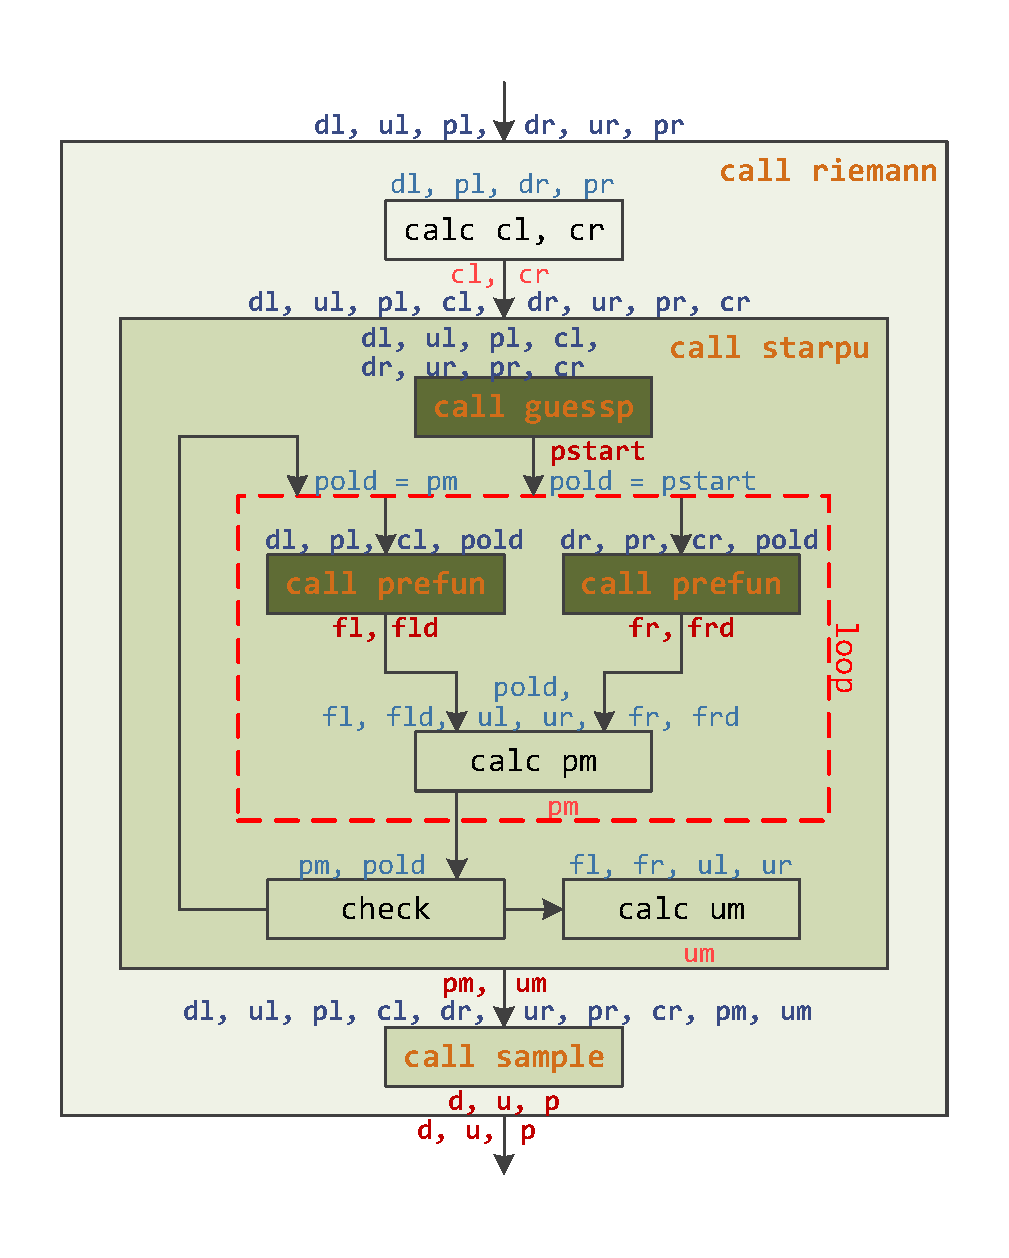
\includegraphics[width=0.5\textwidth]{pics/text_4_vec_riemann/pic_functions.pdf}
\singlespacing
\captionstyle{center}\caption{Схема потока данных в римановском решателе}
\label{fig:text_4_vec_riem_functions}
\end{figure}

Библиотека NUMERICA реализована на языке FORTRAN, поэтому векторизация данного кода с использованием функций-интринсиков\label{term:intrinsic5} напрямую невозможна, поэтому использовалась портированная на язык программирования C версия кода.

На Рис.~\ref{fig:text_4_vec_riem_functions} показана схема работы римановского решателя с обозначенными потоками данных и вызовами всех входящих в реализацию функций.
Функция \texttt{riemann} осуществляет вычисление скорости звука справа и слева, выполняет проверку на образование вакуума и последовательно вызывает функции \texttt{starpu} и \texttt{sample}.
Функция \texttt{starpu} вычисляет значения скорости и давления в среднем регионе между левой и правой волнами (star region), при этом функция содержит цикл с неизвестным количеством итераций для решения нелинейного уравнения итерационным методом Ньютона, внутри которого расположены вызовы других функций (\texttt{prefun}).
Функции \texttt{guessp} и \texttt{prefun} содержат только арифметические вычисления и простые условия и являются наиболее простыми с точки зрения векторизации.
Наконец последняя функция \texttt{sample} определяет окончательную конфигурацию разрыва путем вычисления множества условий.
Эта функция содержит очень разветвленное управление, вложенность условий в ней достигает четырех, что затрудняет применение векторизации.

В процессе счета с помощью численных методов, базирующихся на римановском решателе, выполняется множество вызовов функции \texttt{riemann} с различными наборами входных данных (на каждой итерации счета выполняется один вызов для каждой грани каждой ячейки расчетной сетки).
Так как функция \texttt{riemann} является чистой, то вызовы для разных наборов входных данных (\texttt{dl}, \texttt{ul}, \texttt{pl}, \texttt{dr}, \texttt{ur}, \texttt{pr}) являются независимыми и возникает желание объединения вызовов с целью эффективного задействования векторных (поэлементных) инструкций.
В качестве такого объединенного вызова будем рассматривать функцию, в которую вместо атомарных данных типа \texttt{float} будут подаваться соответствующие векторы, содержащие по 16 элементов.
\begin{equation}\label{eqn:text_4_vec_riem_riemann_16}
\overline{U}_l = [\overline{d}_l, \overline{u}_l, \overline{p}_l], \ 
\overline{U}_r = [\overline{d}_r, \overline{u}_r, \overline{p}_r], \ 
\overline{U} = [\overline{d}, \overline{u}, \overline{p}] = riem(\overline{U}_l, \overline{U}_r)
\end{equation}

В \eqref{eqn:text_4_vec_riem_riemann_16} все переменные $\overline{d}_l$, $\overline{u}_l$, $\overline{p}_l$, $\overline{d}_r$, $\overline{u}_r$, $\overline{p}_r$, $\overline{d}$, $\overline{u}$, $\overline{p}$ являются векторами длины 16.
Например, вектор $\overline{d}$ содержит 16 значений плотности газа, полученных при решении 16 задач Римана, объединенных в один вызов.
Аналогично с другими переменными.
Векторизация простой функции \texttt{prefun} с использованием простого слияния ветвей исполнения по условию\label{term:meth_vec_merge3} с проверкой масок на пустоту\label{term:meth_vec_check2}, а также с объединением масок\label{term:meth_vec_union2}, уже рассматривалась в разделе \ref{sec:text_4_comb_mask_analyze}.
В этом разделе нас интересует функция \texttt{starpu}, которая содержит плоский цикл, телом которого является цикл с непостоянным количеством итераций.

\subsubsection{Векторизация гнезда циклов}

Рассмотрим исходную реализацию скалярной версии функции \texttt{starpu}, представленную на листинге~\ref{lst:text_4_vec_riem_starpu}.

\begin{lstlisting}[caption={Оригинальная версия функции \texttt{starpu}.},label={lst:text_4_vec_riem_starpu}]
void starpu(float dl, float ul, float pl, float cl,
            float dr, float ur, float pr, float cr, float &p, float &u)
{
    const int nriter = 20;
    const float tolpre = 1.0e-6;
    float change, fl, fld, fr, frd, pold, pstart, udiff;

    guessp(dl, ul, pl, cl, dr, ur, pr, cr, pstart);
    pold = pstart;
    udiff = ur - ul;

    int i = 1;
    for ( ; i <= nriter; i++)
    {
        prefun(fl, fld, pold, dl, pl, cl);
        prefun(fr, frd, pold, dr, pr, cr);
        p = pold - (fl + fr + udiff) / (fld + frd);
        change = 2.0 * abs((p - pold) / (p + pold));

        if (change <= tolpre) break;
        if (p < 0.0) p = tolpre;

        pold = p;
    }

    if (i > nriter)
    {
        cout << "divergence in Newton-Raphson iteration" << endl;
        exit(1);
    }

    u = 0.5 * (ul + ur + fr - fl);
}
\end{lstlisting}

Цикл, расположенный в строках 13-24 кроме неизвестного количества итераций содержит также операторы передачи управления (\texttt{if}, \texttt{break}) и вызовы функций \texttt{prefun}, что также усложняет его векторизацию.
Перед выполнением векторизации этот цикл необходимо преобразовать в предикатную форму\label{term:predicate_view3}, в которой тело не должно содержать операций перехода.

\begin{lstlisting}[caption={Векторизованная версия функции \texttt{starpu}.},label={lst:text_4_vec_riem_starpu_vec}]
void starpu_16(__m512 dl, __m512 ul, __m512 pl, __m512 cl,
               __m512 dr, __m512 ur, __m512 pr, __m512 cr,
               __m512 *p, __m512 *u)
{
    ...
    two = SET1(2.0); tolpre = SET1(1.0e-6); tolpre2 = SET1(5.0e-7);
    udiff = SUB(ur, ul);

    guessp_16(dl, ul, pl, cl, dr, ur, pr, cr, &pold);

    // Start with full mask.
    m = 0xFFFF;

    for (; (iter <= nriter) && (m != 0x0); iter++)
    {
        prefun_16(&fl, &fld, pold, dl, pl, cl, m);
        prefun_16(&fr, &frd, pold, dr, pr, cr, m);
        *p = _mm512_mask_sub_ps(*p, m, pold,
                 _mm512_mask_div_ps(z, m,
                     ADD(ADD(fl, fr), udiff), ADD(fld, frd)));
        change = ABS(_mm512_mask_div_ps(z, m,
                         SUB(*p, pold), ADD(*p, pold)));
        cond_break = _mm512_mask_cmp_ps_mask(m, change,
                         tolpre2, _MM_CMPINT_LE);
        m &= ~cond_break;
        cond_neg = _mm512_mask_cmp_ps_mask(m, *p, z, _MM_CMPINT_LT);
        *p = _mm512_mask_mov_ps(*p, cond_neg, tolpre);
        pold = _mm512_mask_mov_ps(pold, m, *p);
    }

    if (iter > nriter)
    {
        cout << "divergence in Newton-Raphson iteration" << endl;
        exit(1);
    }

    *u = MUL(SET1(0.5), ADD(ADD(ul, ur), SUB(fr, fl)));
}
\end{lstlisting}

Запишем цикл в виде, при котором все инструкции цикла выполняются под своими предикатами, и выполнение цикла прерывается при условии обнуления всех предикатов \cite{Krzikalla2026Vec}.
При этом стоит заметить, что вызовы функций \texttt{prefun} также должны обладать соответствующими предикатами.
После преобразования тела цикла в предикатную форму, он может быть векторизован, после чего предикаты инструкций заменятся на векторные регистры-маски (именно в этом месте появляется дополнительный параметр векторизованной функции \texttt{prefun} в виде маски).
Результат векторизации функции \texttt{starpu} представлен на листинге~\ref{lst:text_4_vec_riem_starpu_vec}.

В строке 12 видна изначальная инициализация полной маски выполнения векторизованных итераций цикла.
По мере работы цикла маска истощается (строка 25), и при полном ее обнулении цикл завершает работу.

Стоит отметить, что векторизация цикла с неизвестным числом итераций может быть довольно опасной, так как количество итераций векторизованного цикла равно максимуму из количеств итераций циклов из 16 объединяемых вызовов оригинальной невекторизованной функции.
При большой разнице в количестве итераций оригинального кода возникает падение эффективности, связанное с низкой плотностью масок\label{term:vector_mask_density4} исполняемых инструкций.

\subsubsection{Анализ результатов векторизации гнезда циклов и всего римановского решателя}

Перед началом оптимизации программного кода римановского решателя был выполнен сбор профиля исполнения\label{term:execution_profile2}, который показал, что время исполнения распределено между отдельными функциями согласно диаграмме, представленной на рис.~\ref{fig:text_4_vec_riem_exe_prof}.

\begin{figure}
\centering
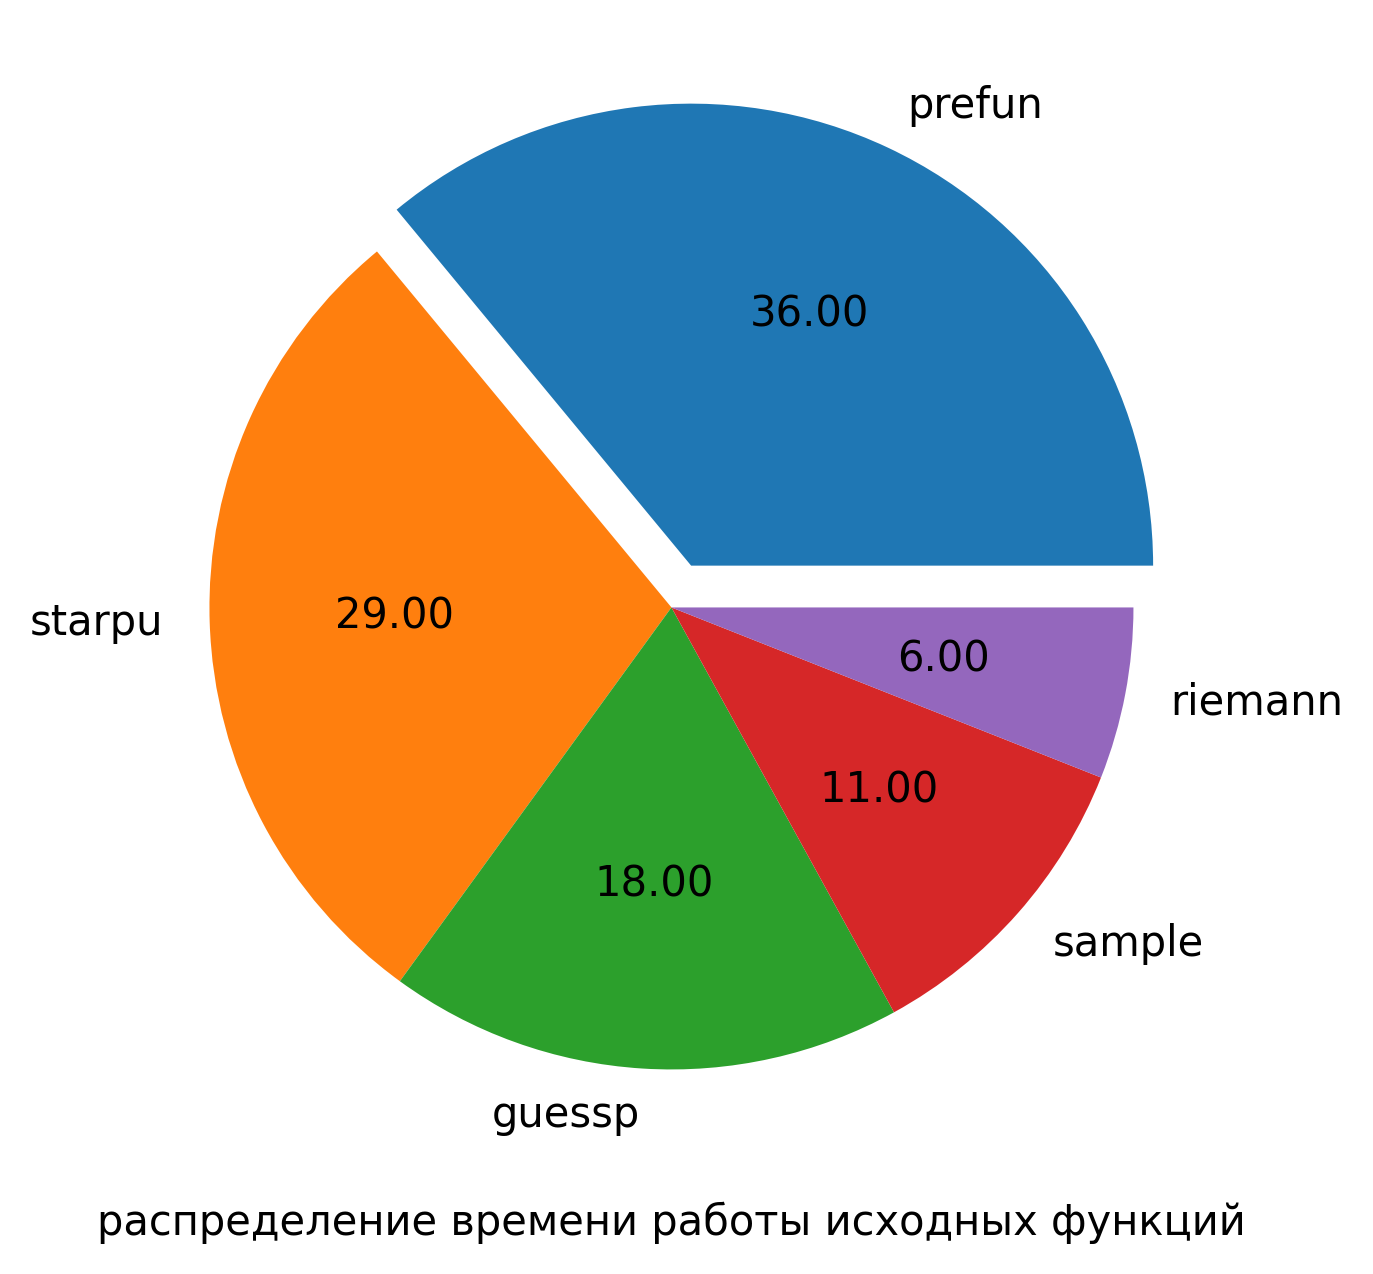
\includegraphics[width=0.5\textwidth]{pics/text_4_vec_riemann/exe_prof.png}
\singlespacing
\captionstyle{center}\caption{Распределение времени выполнения римановского решателя между отдельными функциями.}
\label{fig:text_4_vec_riem_exe_prof}
\end{figure}

Для сбора профиля исполнения исходная программа была скомпилирована с запретом оптимизации подстановки тела функции в точку вызова.
Таким образом, на диаграмме отмечено чистое время выполнения функций без учета вложенных вызовов.
Из диаграммы видно, что наибольшая доля времени исполнения приходится на функцию \texttt{prefun} (36\%), содержащую простой программный контекст с одним условием.
Также значительная часть времени исполнения приходится на функцию \texttt{starpu} (29\%), содержащую гнездо циклов с неизвестным числом итераций.
Оставшееся время делится между тремя другими функциями \texttt{guessp} (18\%), \texttt{sample} (11\%), \texttt{riemann} (6\%).

Для всех функций римановкого решателя была выполнена векторизация, полный программный код векторизованного решателя доступен в \cite{riemannvecGithub}.
Тестирование производительности выполнялось на массивах входных данных, собранных при решении стандартных тестовых задач: задача Сода, задача Лакса, задача о слабой ударной волне, задача Эйнфельдта, задача Вудворда-Колелла, задача Шу-Ошера и других \cite{Bulat2015VecRiemann}.

На диаграмме рис.~\ref{fig:text_4_vec_riemann_perf} показан эффект от применения различных оптимизаций к каждой из рассматриваемых функций, а также суммарное ускорение, полученное вследствие векторизации.

\begin{figure}
\centering
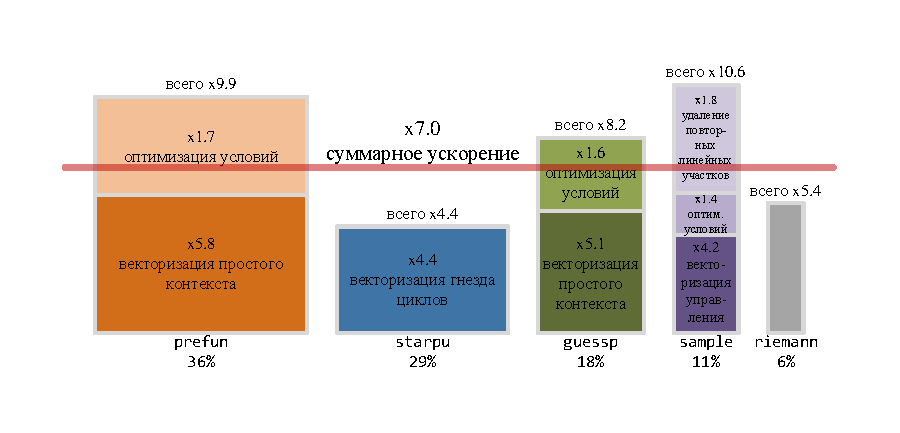
\includegraphics[width=1.0\textwidth]{pics/text_4_vec_riemann/pic_perf.pdf}
\singlespacing
\captionstyle{center}\caption{Диаграмма ускорения отдельных функций и суммарного ускорения римановского решателя.}
\label{fig:text_4_vec_riemann_perf}
\end{figure}

Можно отметить, что эффект от векторизации простого контекста варьируется в пределах от 5,1 до 5,8 раза (для функций \texttt{guessp} и \texttt{prefun}).
Также следует отметить существенный эффект от оптимизации условий (проверка на пустоту маски предикатов, под которой находится выполнение блока операций).
Это довольно простое преобразование, приводит к ускорению кода от 1,4 до 1,7 раз (для функций \texttt{sample} и \texttt{prefun}) в зависимости от того, насколько близкими являются условия с соседних итераций векторизуемого цикла.

Отдельно на диаграмме выделен эффект от применения оптимизации замены переменных, позволившей в 1,8 раз ускорить функцию \texttt{sample} путем слияния двух поддеревьев графа потока управления\label{term:graph_cfg3} (то есть было выполнено удаление дублирующих линейных участков).

В результате применения всех описанных оптимизаций удалось достичь ускорения отдельных участков выполнения программы в 10 и более раз, а суммарное ускорение всего римановского решателя составило 7 раз (отмечено красной линией на рис.~\ref{fig:text_4_vec_riemann_perf}).
